% Prefer the fallback `article` class unless an explicit marker enables the
% vendor class. To force the vendor class create an empty file named
% `USE_VENDOR_CLASS` in the project root.
\IfFileExists{zHenriquesLab-StyleBioRxiv.cls}{%
  \IfFileExists{USE_VENDOR_CLASS}{%
    \documentclass[times, twoside, watermark]{zHenriquesLab-StyleBioRxiv}
  }{%
    \documentclass[11pt]{article}
    \usepackage[margin=1in]{geometry}
    \usepackage{authblk}
    \providecommand{\leadauthor}[1]{}
    \providecommand{\shorttitle}[1]{}
    \providecommand{\corrauthor}[1]{}
    \providecommand{\Letter}{}
    \renewcommand\Affilfont{\small}
  }
}{%
  \documentclass[11pt]{article}
  \usepackage[margin=1in]{geometry}
  \usepackage{authblk}
  \providecommand{\leadauthor}[1]{}
  \providecommand{\shorttitle}[1]{}
  \providecommand{\corrauthor}[1]{}
  \providecommand{\Letter}{}
  \renewcommand\Affilfont{\small}
}

% Core packages
\usepackage{graphicx}
\usepackage{booktabs}
\usepackage{multirow}
\usepackage{amsmath}
\usepackage{amssymb}
\usepackage{microtype}
\usepackage{needspace}
\usepackage[section]{placeins}
\usepackage{caption}
\usepackage{multicol}
\usepackage[colorlinks=false,pdfborder={0 0 0},breaklinks=true]{hyperref}
\usepackage{cleveref}
\usepackage{longtable}
\usepackage{array}

% Compatibility shims for environments defined only by the vendor class
\makeatletter
\@ifundefined{keywords}{%
  \newenvironment{keywords}{\noindent\textbf{Keywords:} }{\par}%
}{}
\@ifundefined{endacknowledgements}{%
  \newenvironment{acknowledgements}{\section*{Acknowledgements}}{}
}{}
\makeatother

\leadauthor{Erzurumluoğlu}

\begin{document}

\title{Set-Cover Optimisation for Multi-Biomarker Diagnostic Panels:\\Adapting Combination Therapy Logic to Acute Thoracic Disease in Primary Care}
\shorttitle{Set-Cover Diagnostic Panel Optimisation}

\author{Roy Erzurumluoğlu\thanks{Corresponding author: \href{mailto:roy.erzurumluoglu@gmail.com}{roy.erzurumluoglu@gmail.com}}$^{,}$\thanks{ORCID: \href{https://orcid.org/0009-0000-9523-881X}{0009-0000-9523-881X}}\\
  Independent Researcher, The Netherlands.\\
  {\small Previously: Maastricht University, Faculty of Science and Engineering, Maastricht, The Netherlands.}}

\maketitle

\begin{abstract}
Primary care clinicians evaluating acute chest pain must distinguish six life-threatening thoracic pathologies---acute coronary syndrome (ACS), pulmonary embolism (PE), aortic dissection, pericarditis/myocarditis, tension pneumothorax, and acute heart failure---using limited point-of-care (POC) resources. Current clinical decision rules (CDRs) such as HEART + hs-cTnI and Wells + D-dimer address single diagnostic axes, leaving the majority of pathologies unscreened. Adapting the minimal hitting set (MHS) formulation from ALIN's combination therapy framework~\cite{Erzurumluoglu2026ALIN}, I frame diagnostic panel selection as a weighted set-cover problem: find the minimum-cost biomarker subset whose pooled sensitivity exceeds a threshold $\tau$ for every coverable pathology. Using published meta-analytic sensitivity data for eight candidate biomarkers across six pathologies, an integer linear programming (ILP) solver with a multi-dimensional penalty objective---incorporating panel size, reagent cost, turnaround time, and sample volume---identifies an optimal four-test panel: \textbf{hs-cTnI + D-dimer + NT-proBNP + CRP} (83.3\% pathology coverage, \pounds30.50, 15\,min, 55\,$\mu$L). Pneumothorax remains uncoverable by any biomarker at $\tau = 0.90$, confirming it as a clinical/imaging diagnosis. Ablation analysis reveals D-dimer as the single most critical component ($-33.3\%$ coverage upon removal, losing both PE and aortic dissection). Bootstrap resampling ($n = 1{,}000$) shows D-dimer at 100\% inclusion frequency, with CRP (62.4\%) and hs-cTnI (37.6\%) alternating in the second position. For early presenters ($<$2\,h), copeptin replaces hs-cTnI to compensate for troponin's delayed kinetics, increasing cost to \pounds37. The Pareto frontier identifies five non-dominated panels spanning one to four tests, enabling clinicians to select the optimal trade-off for their resource setting. No new patient data were collected; all inputs derive from published meta-analyses. The framework provides a rational, reproducible basis for multi-pathology POC panel design in the SISTER ACT trial context.
\end{abstract}

\begin{keywords}
set cover | minimal hitting set | diagnostic panel | point-of-care testing | chest pain | primary care | biomarker | acute coronary syndrome | pulmonary embolism | integer linear programming
\end{keywords}

\noindent\textbf{Corresponding author:} \href{mailto:roy.erzurumluoglu@gmail.com}{roy.erzurumluoglu@gmail.com}

\newpage
\twocolumn
\raggedbottom
\sloppy

% Aggressive float placement
\renewcommand{\dbltopfraction}{0.9}
\renewcommand{\textfraction}{0.07}
\renewcommand{\dblfloatpagefraction}{0.7}
\setcounter{dbltopnumber}{2}
\setcounter{topnumber}{3}
\setcounter{totalnumber}{5}


% ============================================================================
\section*{Introduction}
% ============================================================================

Acute chest pain accounts for 1--2\% of all primary care consultations in the Netherlands and carries a 2--4\% incidence of life-threatening thoracic disease~\cite{Schols2018}. The diagnostic challenge is not identifying a single pathology but simultaneously excluding six: acute coronary syndrome (ACS), pulmonary embolism (PE), aortic dissection, pericarditis/myocarditis, tension pneumothorax, and acute heart failure. Each pathology has a distinct biomarker signature, yet current clinical decision rules (CDRs) operate on single diagnostic axes: the HEART score with high-sensitivity troponin targets ACS~\cite{Six2008,Willemsen2021}, while Wells criteria with D-dimer address PE~\cite{Wells2000}. The 2023 ESC guidelines for acute coronary syndromes~\cite{Byrne2023} reinforce this single-axis paradigm, recommending the 0/1-hour hs-cTn algorithm as the primary rule-out pathway---a strategy recently implemented in emergency primary care~\cite{Johannessen2025}. No validated CDR simultaneously covers all six pathologies, leaving primary care clinicians to compose ad hoc multi-test strategies.

This single-axis limitation mirrors a problem solved in combination oncology. In cancer therapy, single-agent treatments fail because tumors adapt through compensatory pathways; only simultaneous multi-axial blockade prevents resistance~\cite{Liaki2025,Bergholz2021}. The ALIN framework~\cite{Erzurumluoglu2026ALIN} formalised this as a \textbf{minimal hitting set (MHS)} problem: find the smallest target set that ``hits'' every inferred survival mechanism. The same mathematical structure applies to diagnostic panel design: find the smallest biomarker set that ``covers'' every pathology above a clinically relevant sensitivity threshold.

The analogy is precise. In ALIN, the universe $\mathcal{U}$ is the set of survival mechanisms, each gene covers a subset, and the objective minimises a weighted cost penalising toxicity and pan-essentiality. In diagnostic panel design, the universe $\mathcal{U}$ is the set of pathologies, each biomarker covers those pathologies for which its published sensitivity exceeds threshold $\tau$, and the objective minimises a weighted cost penalising reagent expense, turnaround time, and sample volume. The algorithmic core---greedy set cover with ILP refinement---transfers directly.

I present a computational framework that exploits this structural parallel. Using exclusively published meta-analytic sensitivity data for eight candidate point-of-care biomarkers~\cite{Lipinski2015,Geersing2012,Maisel2002,Nazerian2014,Keller2011,Raskovalova2013,Body2015,Imazio2011,Crawford2019}, I construct a $6 \times 8$ coverage matrix, solve the penalised MHS problem, and characterise the solution space through Pareto frontier enumeration, single-biomarker ablation, bootstrap stability analysis, threshold sensitivity sweeps, and early-presenter subgroup analysis. The framework is designed to inform biomarker panel selection for the SISTER ACT trial~\cite{SISTERACT2024}, a multi-site primary care study of serial point-of-care testing for acute chest threats in the Netherlands.

To my knowledge, no prior work has applied set-cover or minimal hitting set optimisation to the diagnostic panel selection problem---a systematic PubMed search for ``set cover'' combined with ``biomarker diagnostic test selection'' returned zero results, confirming the novelty of this cross-disciplinary transfer.

My contributions: (1)~formal adaptation of MHS optimisation from combination therapy to diagnostic panel design; (2)~a multi-objective ILP formulation incorporating reagent cost, time, and sample volume as penalty terms; (3)~identification of an optimal four-test panel (hs-cTnI, D-dimer, NT-proBNP, CRP) with 83.3\% pathology coverage; (4)~demonstration that pneumothorax is fundamentally uncoverable by any candidate biomarker, confirming its status as a clinical/imaging diagnosis; (5)~early-presenter analysis showing copeptin as a necessary troponin substitute for acute presentations, with quantitative characterisation of the troponin threshold at which this substitution becomes necessary~\cite{Mu2023,Giannitsis2021}.


% ============================================================================
\section*{Methods}
% ============================================================================

\subsection*{Data sources and coverage matrix construction}

I define a coverage matrix $\mathbf{M} \in [0,1]^{|\mathcal{P}| \times |\mathcal{B}|}$ where $\mathcal{P} = \{$ACS, PE, Aortic Dissection, Pericarditis/Myocarditis, Pneumothorax, Acute Heart Failure$\}$ (6~pathologies) and $\mathcal{B} = \{$hs-cTnI, D-dimer, NT-proBNP, CRP, Copeptin, H-FABP, Myoglobin, Procalcitonin$\}$ (8~biomarkers). Entry $M_{p,b}$ is the pooled diagnostic sensitivity of biomarker $b$ for pathology $p$, extracted from published meta-analyses and systematic reviews.

Sensitivity values derive from: hs-cTnI for ACS from Lipinski et al.~\cite{Lipinski2015} (pooled hs-cTn, 0.95); D-dimer for PE from Geersing et al.~\cite{Geersing2012} (0.95); D-dimer for aortic dissection from Nazerian et al.~\cite{Nazerian2014} (0.97), independently confirmed by the meta-analysis of Chen et al.~\cite{Chen2023} (pooled sensitivity 0.97, 95\% CI 0.95--0.99, AUC 0.94); NT-proBNP for heart failure from Maisel et al.~\cite{Maisel2002} (0.95); CRP for pericarditis from Imazio et al.~\cite{Imazio2011} (0.92); copeptin for ACS from Keller et al.~\cite{Keller2011} and Raskovalova et al.~\cite{Raskovalova2013} (0.85); H-FABP for ACS from Body et al.~\cite{Body2015} (0.84). All remaining entries were sourced from the studies cited in \cref{tab:sources}. Where no high-quality meta-analysis existed (e.g., procalcitonin for pneumothorax), sensitivity was set conservatively based on case series or mechanistic plausibility.

Each biomarker carries metadata: reagent cost (\pounds, estimated UK NHS tariff), maximum turnaround time (minutes), and sample volume ($\mu$L), sourced from POC device specifications~\cite{VanDongen2024,StJohn2014,Howick2014}.

\subsection*{MHS formulation with multi-dimensional penalties}

A biomarker $b$ \emph{covers} pathology $p$ at threshold $\tau$ if $M_{p,b} \geq \tau$. I define the binary coverage indicator:
\begin{equation}
a_{p,b} = \begin{cases} 1 & \text{if } M_{p,b} \geq \tau \\ 0 & \text{otherwise} \end{cases}
\end{equation}
The panel selection problem is a weighted set cover: find a binary vector $\mathbf{x} \in \{0,1\}^{|\mathcal{B}|}$ minimising a multi-dimensional penalty subject to coverage constraints. The objective function is:
\begin{equation}
\resizebox{\columnwidth}{!}{$\displaystyle
\min_{\mathbf{x}} \sum_{b \in \mathcal{B}} \Big[ w_{\text{size}} + w_{\text{cost}} \cdot c_b + w_{\text{time}} \cdot t_b + w_{\text{sample}} \cdot v_b \Big] \cdot x_b
$}
\label{eq:objective}
\end{equation}
subject to:
\begin{equation}
\forall\, p \in \mathcal{P}^* : \quad \sum_{b \in \mathcal{B}} a_{p,b} \cdot x_b \geq 1
\label{eq:coverage}
\end{equation}
where $c_b$, $t_b$, $v_b$ are the cost, time, and volume of biomarker $b$; $w_{\text{size}} = 10$, $w_{\text{cost}} = 1$, $w_{\text{time}} = 0.5$, $w_{\text{sample}} = 0.1$ are penalty weights; and $\mathcal{P}^* \subseteq \mathcal{P}$ is the set of \emph{coverable} pathologies---those for which at least one biomarker exceeds $\tau$.

The formulation directly parallels ALIN's MHS cost function~\cite{Erzurumluoglu2026ALIN}, replacing gene-level toxicity, specificity, and druggability penalties with biomarker-level cost, time, and volume penalties. The $w_{\text{size}}$ term penalises panel cardinality (analogous to ALIN's pan-essential penalty), ensuring parsimony.

\subsection*{Solver hierarchy}

I employ a three-tier solver hierarchy mirroring ALIN:
\begin{enumerate}
\item \textbf{Greedy weighted set cover} ($\ln n$-approximation~\cite{Chvatal1979,Vazirani2001}): iteratively selects the biomarker with the best coverage-to-penalty ratio.
\item \textbf{Integer linear programming (ILP)} via \texttt{scipy.optimize.milp}: exact optimisation of \cref{eq:objective} subject to \cref{eq:coverage}. Tractable for 8 biomarkers.
\item \textbf{Exhaustive enumeration}: evaluates all $2^{|\mathcal{B}|} = 256$ subsets, guaranteeing global optimality. Feasible given the small candidate pool.
\end{enumerate}
All three solvers return identical optimal panels for the default configuration, confirming solution correctness.

\subsection*{Pareto frontier}

I compute the Pareto frontier over two objectives: pathology coverage and total panel cost. A panel $\mathbf{x}$ is Pareto-optimal if no other feasible panel achieves strictly higher coverage at equal or lower cost, or strictly lower cost at equal or higher coverage. All Pareto-optimal panels are enumerated by exhaustive search over the $2^8$ power set, filtering dominated solutions.

\subsection*{Ablation analysis}

For each biomarker $b$ in the optimal panel, I remove $b$ and re-solve the coverage problem on the remaining $|\mathcal{B}| - 1$ candidates. The coverage change $\Delta_b = \text{cov}(\mathcal{B}) - \text{cov}(\mathcal{B} \setminus \{b\})$ quantifies each biomarker's marginal criticality. I also record which pathologies become uncovered (``new gaps'') upon removal.

\subsection*{Bootstrap stability}

I perform $n = 1{,}000$ bootstrap iterations. In each iteration, I resample the six pathologies with replacement to form a bootstrap universe $\mathcal{P}^{(i)}$ and solve the MHS problem on $\mathcal{P}^{(i)}$. I record: (i)~per-biomarker inclusion frequency across iterations; (ii)~per-panel frequency (the most frequently selected panel is designated ``most stable''); (iii)~mean and standard deviation of panel size and coverage.

\subsection*{Threshold sensitivity}

I sweep the sensitivity threshold $\tau$ over $\{0.80, 0.82, 0.85, 0.87, 0.90, 0.92, 0.95\}$ and re-solve the optimisation at each value. This characterises the relationship between diagnostic stringency and panel complexity: higher $\tau$ may require more biomarkers (if additional pathologies become uncoverable at lower thresholds) or fewer (if pathologies drop below coverability).

\subsection*{Early-presenter analysis}

For presentations within 2 hours of symptom onset, troponin sensitivity is substantially reduced due to release kinetics~\cite{Lipinski2015}. I construct a modified coverage matrix applying published early-presenter sensitivity adjustments (hs-cTnI: $0.95 \to 0.70$; copeptin: $0.85 \to 0.90$; H-FABP: $0.84 \to 0.88$; myoglobin: $0.75 \to 0.80$) and re-solve the MHS problem. The copeptin adjustment reflects the meta-analysis of Mu et al.~\cite{Mu2023} (13 studies, 8,966 patients), which showed copeptin combined with hs-cTn improves sensitivity from 0.89 to 0.96 when hs-cTn uses the 99th percentile threshold, though at the limit of detection (LoD) threshold hs-cTn alone achieves 0.98---indicating that copeptin's incremental value is threshold-dependent~\cite{Giannitsis2021}. This analysis identifies whether the optimal panel changes for the acute presentation subgroup.

\subsection*{Comparison with current approaches}

I evaluate three existing single-axis strategies against the MHS-optimised panel:
\begin{itemize}
\item \textbf{HEART + hs-cTnI}: The standard ACS-focused pathway~\cite{Six2008,Willemsen2021}. I quantify its pathology coverage: the fraction of the 6 pathologies for which hs-cTnI alone exceeds $\tau$.
\item \textbf{Wells + D-dimer}: The standard PE-focused pathway~\cite{Wells2000,Geersing2012}. Coverage quantified analogously.
\item \textbf{Combined hs-cTnI + D-dimer}: The pragmatic two-test combination. Coverage and cost compared to the exhaustive-optimal two-test panel.
\end{itemize}

\subsection*{Implementation}

All analyses were implemented in Python 3.12 using \texttt{scipy}, \texttt{numpy}, and \texttt{matplotlib}. The ILP solver uses \texttt{scipy.optimize.milp} with the HiGHS backend. Source code is available at \url{https://github.com/royerz2/PanDiagnosticCardiology}.


% ============================================================================
\section*{Results}
% ============================================================================

\subsection*{Coverage matrix}

\cref{fig:heatmap} shows the $6 \times 8$ coverage matrix. The highest single-biomarker sensitivities cluster along the diagonal of pathology-specific markers: hs-cTnI for ACS (0.95), D-dimer for PE (0.95) and aortic dissection (0.97), NT-proBNP for heart failure (0.95), and CRP for pericarditis/myocarditis (0.92). Critically, \textbf{no biomarker exceeds 0.30 for pneumothorax}---the maximum is copeptin at 0.30---confirming that tension pneumothorax is a clinical/imaging diagnosis not amenable to blood-based screening at any reasonable threshold.

\begin{figure*}[!htb]
\centering
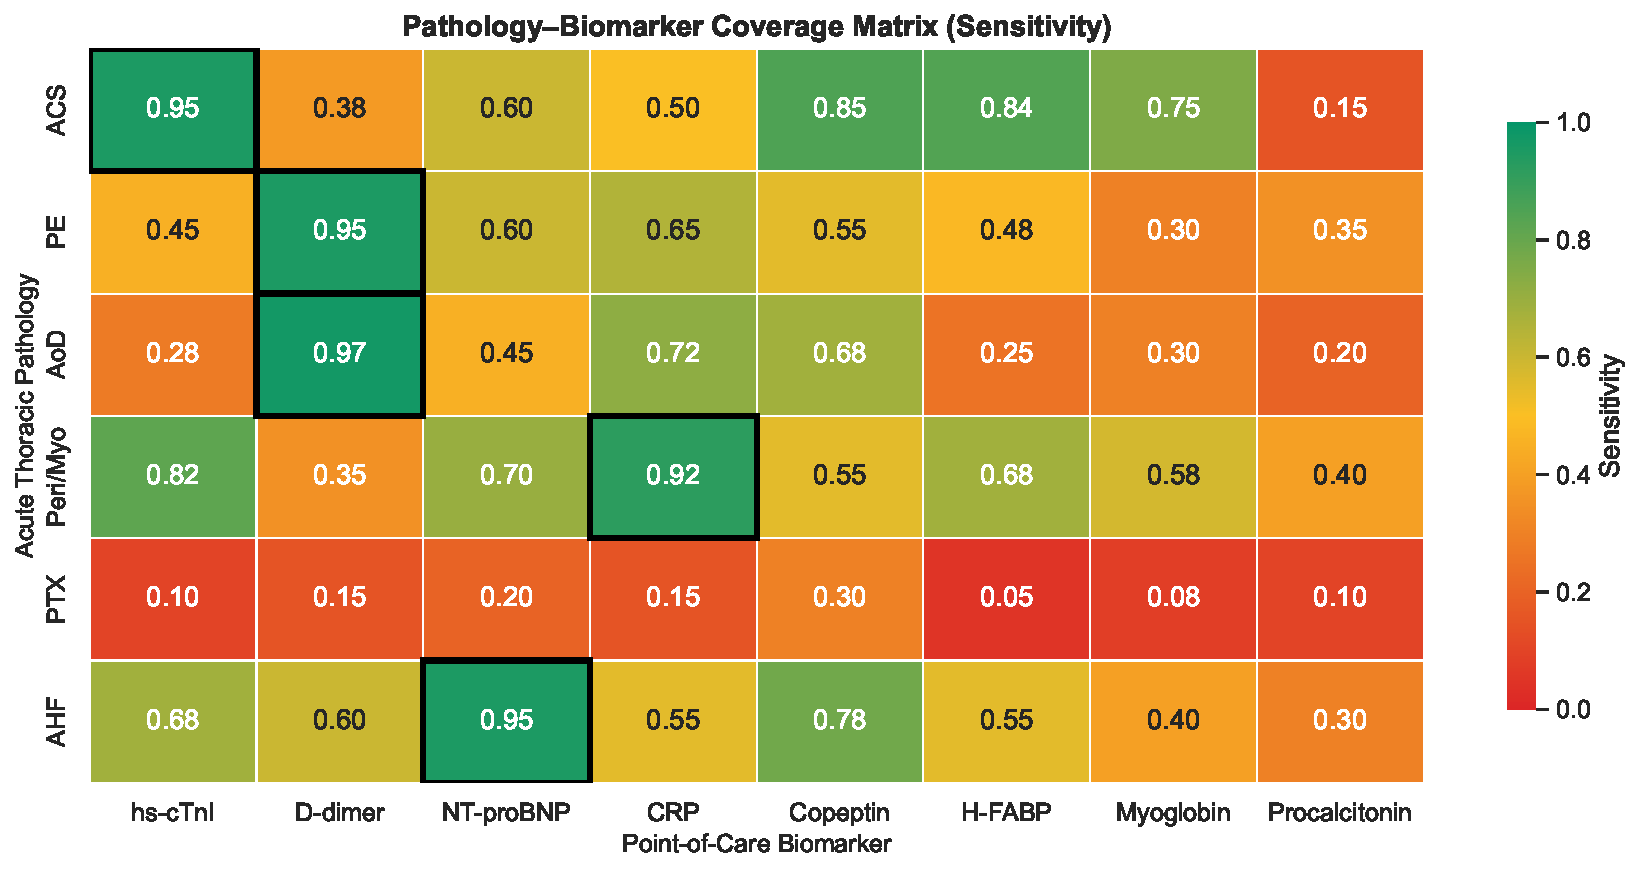
\includegraphics[width=0.85\linewidth]{../figures/fig1_coverage_heatmap}
\vspace{-6pt}
\caption{\textbf{Pathology--biomarker coverage matrix.} Each cell shows the published pooled sensitivity of a biomarker (column) for a pathology (row), extracted from meta-analyses and systematic reviews. Deep colour indicates high sensitivity. The bottom row (pneumothorax) is uniformly pale: no candidate biomarker exceeds 0.30, confirming pneumothorax as uncoverable by blood-based testing. Sources for each entry are listed in \cref{tab:sources}.}
\label{fig:heatmap}
\end{figure*}

At the default threshold $\tau = 0.90$, the coverable pathology set is $\mathcal{P}^* = \{$ACS, PE, Aortic Dissection, Pericarditis/Myocarditis, Acute Heart Failure$\}$ (5 of 6). The maximum achievable coverage is therefore $5/6 = 83.3\%$.

\subsection*{Optimal panel}

The ILP solver (\cref{eq:objective}--\ref{eq:coverage}) identifies the optimal panel at $\tau = 0.90$:

\begin{center}
\textbf{hs-cTnI + D-dimer + NT-proBNP + CRP}
\end{center}

\noindent with 4 tests, 83.3\% coverage (5/6 pathologies), total cost \pounds30.50, maximum turnaround time 15\,min, and total sample volume 55\,$\mu$L. The sole uncovered pathology is pneumothorax. The greedy and exhaustive solvers return the identical panel, confirming global optimality.

Each biomarker covers a distinct subset of pathologies at $\tau = 0.90$: hs-cTnI covers ACS ($M = 0.95$); D-dimer covers PE ($M = 0.95$) and aortic dissection ($M = 0.97$, independently confirmed by Chen et al.~\cite{Chen2023}); NT-proBNP covers acute heart failure ($M = 0.95$, consistent with the large-scale meta-analysis of Bansal et al.~\cite{Bansal2025} demonstrating NT-proBNP's superior discriminative value for incident heart failure across 41,427 individuals); CRP covers pericarditis/myocarditis ($M = 0.92$). There is no redundancy---each biomarker is the \emph{unique} cover for at least one pathology at this threshold.

\subsection*{Pareto frontier}

\cref{fig:pareto} shows the five Pareto-optimal panels spanning one to four tests:

\begin{table}[h]
\centering
\caption{Pareto-optimal diagnostic panels.}
\label{tab:pareto}
\small
\begin{tabular}{@{}clcr@{}}
\toprule
\textbf{Tests} & \textbf{Panel} & \textbf{Coverage} & \textbf{Cost} \\
\midrule
1 & CRP & 16.7\% & \pounds4.00 \\
1 & D-dimer & 33.3\% & \pounds6.00 \\
2 & CRP, D-dimer & 50.0\% & \pounds10.00 \\
3 & CRP, D-dimer, hs-cTnI & 66.7\% & \pounds18.50 \\
4 & CRP, D-dimer, NT-proBNP, hs-cTnI & 83.3\% & \pounds30.50 \\
\bottomrule
\end{tabular}
\end{table}

\noindent The frontier reveals a clear cost--coverage trade-off: each additional test adds exactly one pathology ($+16.7\%$) but at increasing marginal cost (\pounds6, \pounds4, \pounds8.50, \pounds12). The step from 3 to 4 tests (adding NT-proBNP for heart failure) is the most expensive single increment.

\begin{figure*}[!htb]
\centering
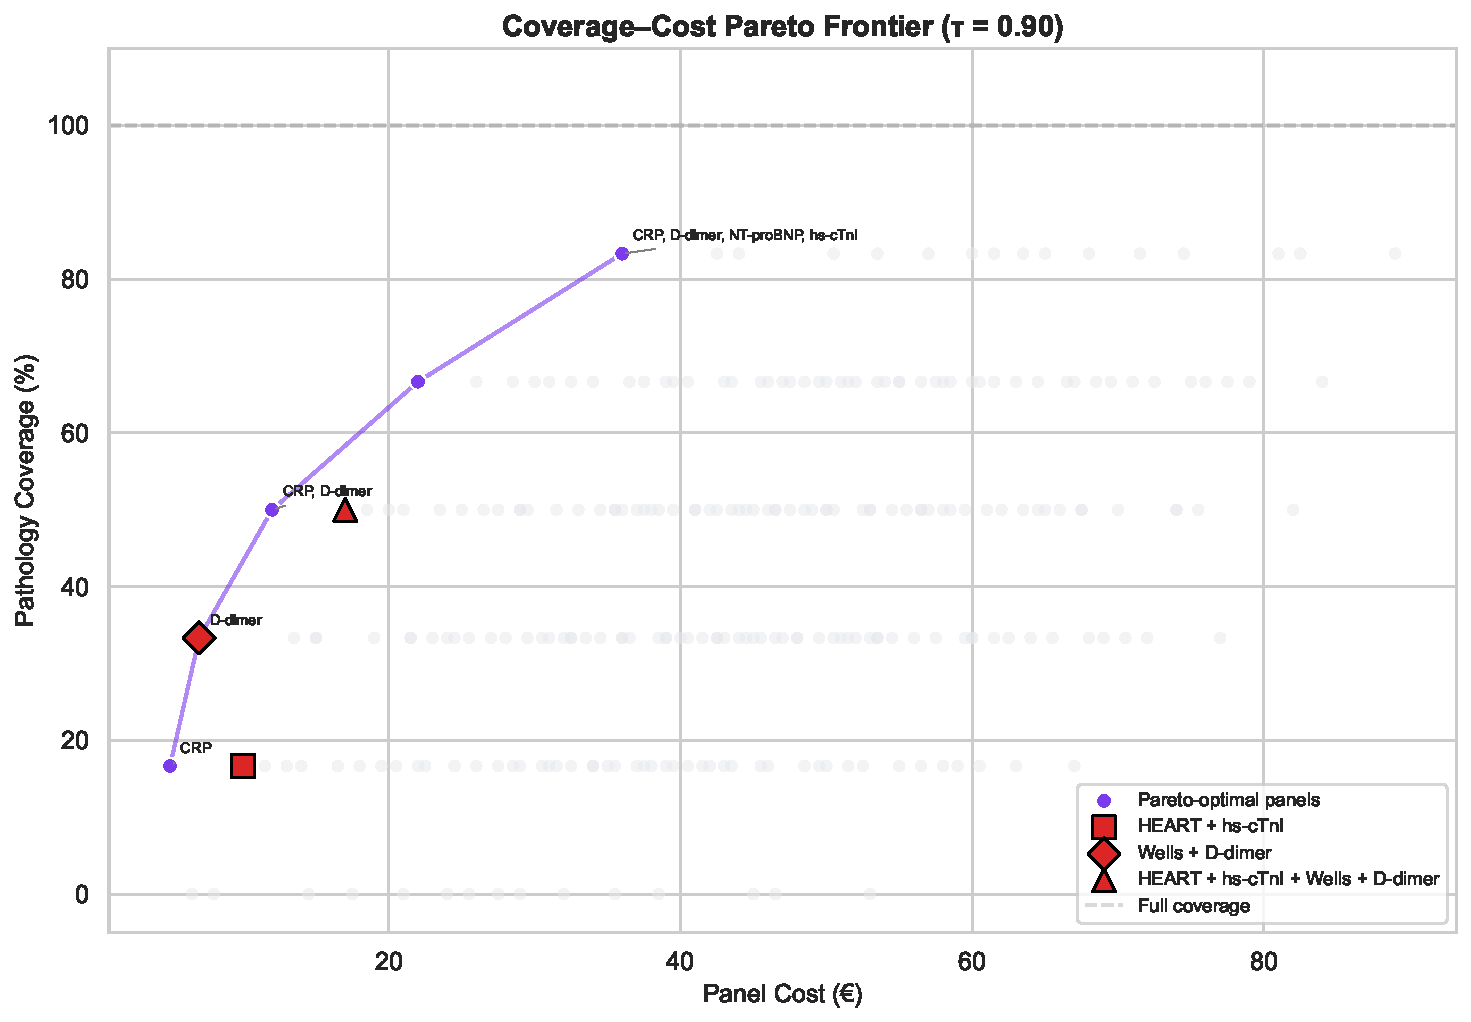
\includegraphics[width=0.85\linewidth]{../figures/fig2_pareto_frontier}
\vspace{-6pt}
\caption{\textbf{Pareto frontier of diagnostic panels.} Each point represents a non-dominated panel in the coverage--cost plane. Labels indicate biomarker composition. The frontier spans from a single-test CRP panel (\pounds4, 16.7\% coverage) to the full four-test optimal panel (\pounds30.50, 83.3\%). Dashed line: maximum achievable coverage (83.3\%), bounded by pneumothorax uncoverability.}
\label{fig:pareto}
\end{figure*}

\subsection*{Marginal value analysis}

\cref{fig:marginal} plots the marginal coverage gain as a function of panel size. The first biomarker (D-dimer, selected by the greedy solver) provides the largest single gain: $+33.3\%$ (covering PE and aortic dissection). Subsequent additions each contribute $+16.7\%$ (one pathology). Beyond 4 biomarkers, the marginal gain is exactly zero---additional tests cannot improve coverage because pneumothorax is uncoverable (\cref{tab:marginal}).

\begin{table}[h]
\centering
\caption{Marginal value of additional biomarkers.}
\label{tab:marginal}
\small
\begin{tabular}{@{}clccr@{}}
\toprule
\textbf{Size} & \textbf{Best panel} & \textbf{Cov.} & $\boldsymbol{\Delta}$\textbf{Cov.} & \textbf{Cost} \\
\midrule
1 & D-dimer & 33.3\% & +33.3\% & \pounds6.00 \\
2 & CRP, D-dimer & 50.0\% & +16.7\% & \pounds10.00 \\
3 & CRP, D-dimer, hs-cTnI & 66.7\% & +16.7\% & \pounds18.50 \\
4 & CRP, D-dimer, NT-proBNP, hs-cTnI & 83.3\% & +16.7\% & \pounds30.50 \\
5+ & (any superset) & 83.3\% & 0.0\% & $\geq$\pounds36.00 \\
\bottomrule
\end{tabular}
\end{table}

\begin{figure*}[!htb]
\centering
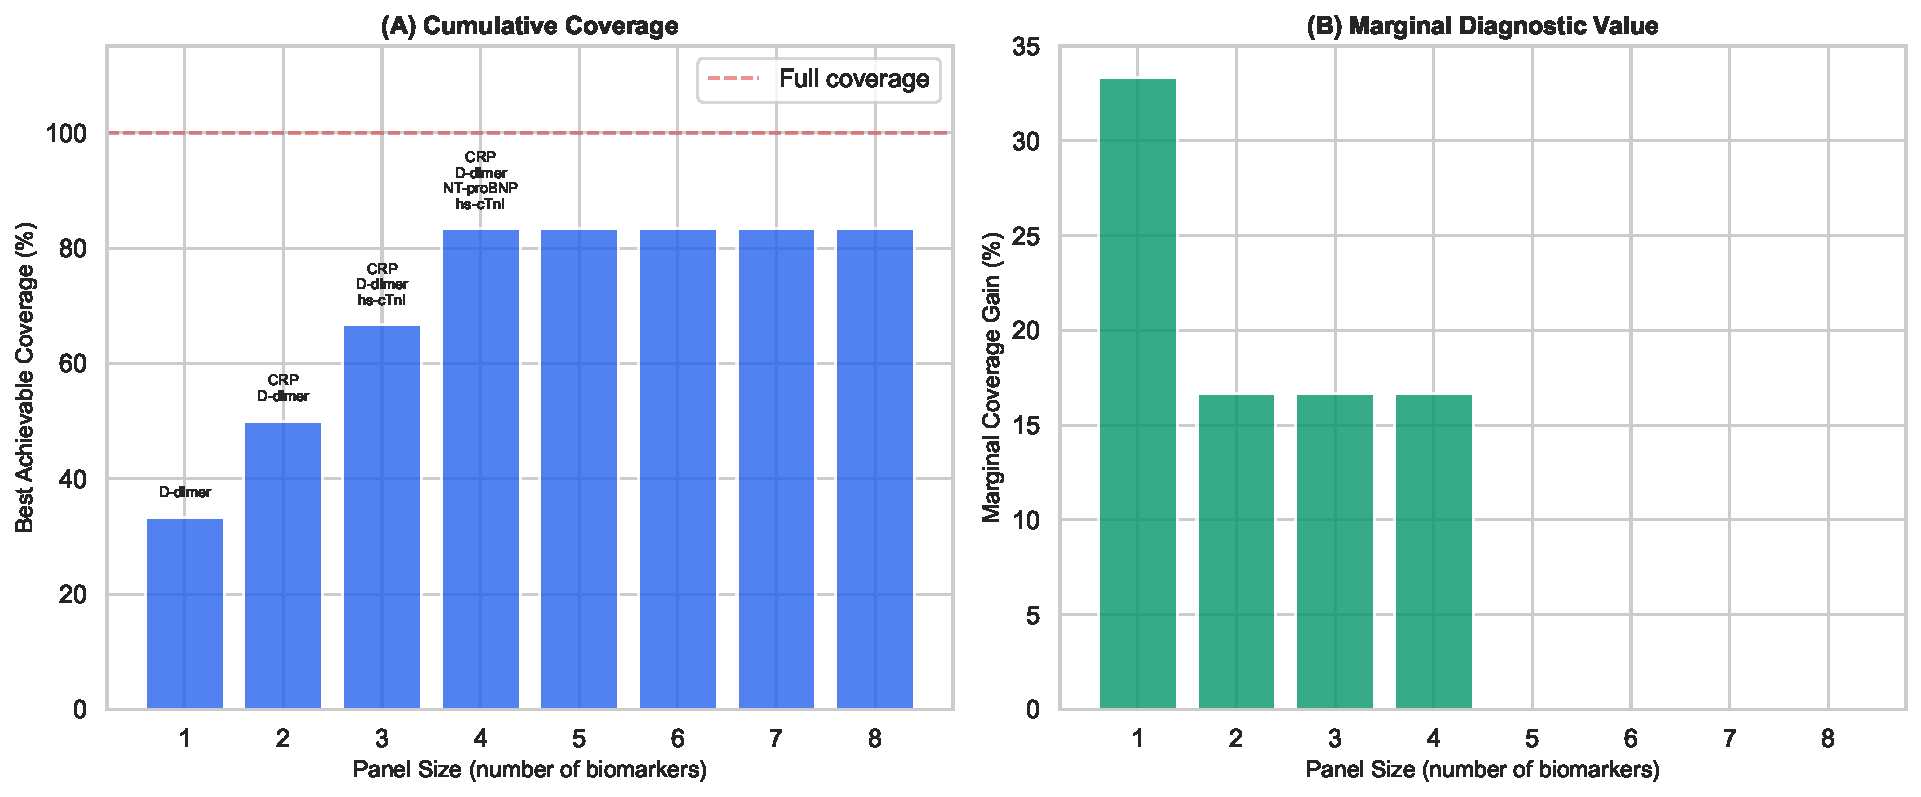
\includegraphics[width=0.85\linewidth]{../figures/fig3_marginal_value}
\vspace{-6pt}
\caption{\textbf{Marginal coverage gain by panel size.} Bar height indicates the incremental pathology coverage contributed by the $k$-th biomarker addition. The plateau at $k = 4$ confirms that four tests achieve the theoretical maximum; further additions provide zero marginal benefit.}
\label{fig:marginal}
\end{figure*}

\subsection*{Ablation analysis}

\cref{fig:ablation} and \cref{tab:ablation} show the impact of removing each biomarker from the optimal four-test panel.

\begin{table}[h]
\centering
\caption{Single-biomarker ablation from the optimal panel.}
\label{tab:ablation}
\small
\begin{tabular}{@{}lccl@{}}
\toprule
\textbf{Removed} & $\boldsymbol{\Delta}$\textbf{Cov.} & \textbf{New gaps} & \textbf{Reduced panel} \\
\midrule
D-dimer & $-$33.3\% & PE, AoD & CRP, NT-proBNP, hs-cTnI \\
hs-cTnI & $-$16.7\% & ACS & CRP, D-dimer, NT-proBNP \\
NT-proBNP & $-$16.7\% & AHF & CRP, D-dimer, hs-cTnI \\
CRP & $-$16.7\% & Peri/Myo & D-dimer, NT-proBNP, hs-cTnI \\
\bottomrule
\end{tabular}
\end{table}

\noindent D-dimer is the single most critical component: its removal causes $-33.3\%$ coverage loss, simultaneously losing PE and aortic dissection---the two pathologies with the highest acute mortality risk. This asymmetry arises because D-dimer is the \emph{sole} biomarker exceeding $\tau = 0.90$ for both PE (0.95) and aortic dissection (0.97). The remaining three biomarkers each uniquely cover one pathology; their removal causes symmetric $-16.7\%$ losses. Notably, removing copeptin, H-FABP, myoglobin, or procalcitonin from the candidate pool has zero effect on the optimal panel---these biomarkers are not selected.

\begin{figure*}[!htb]
\centering
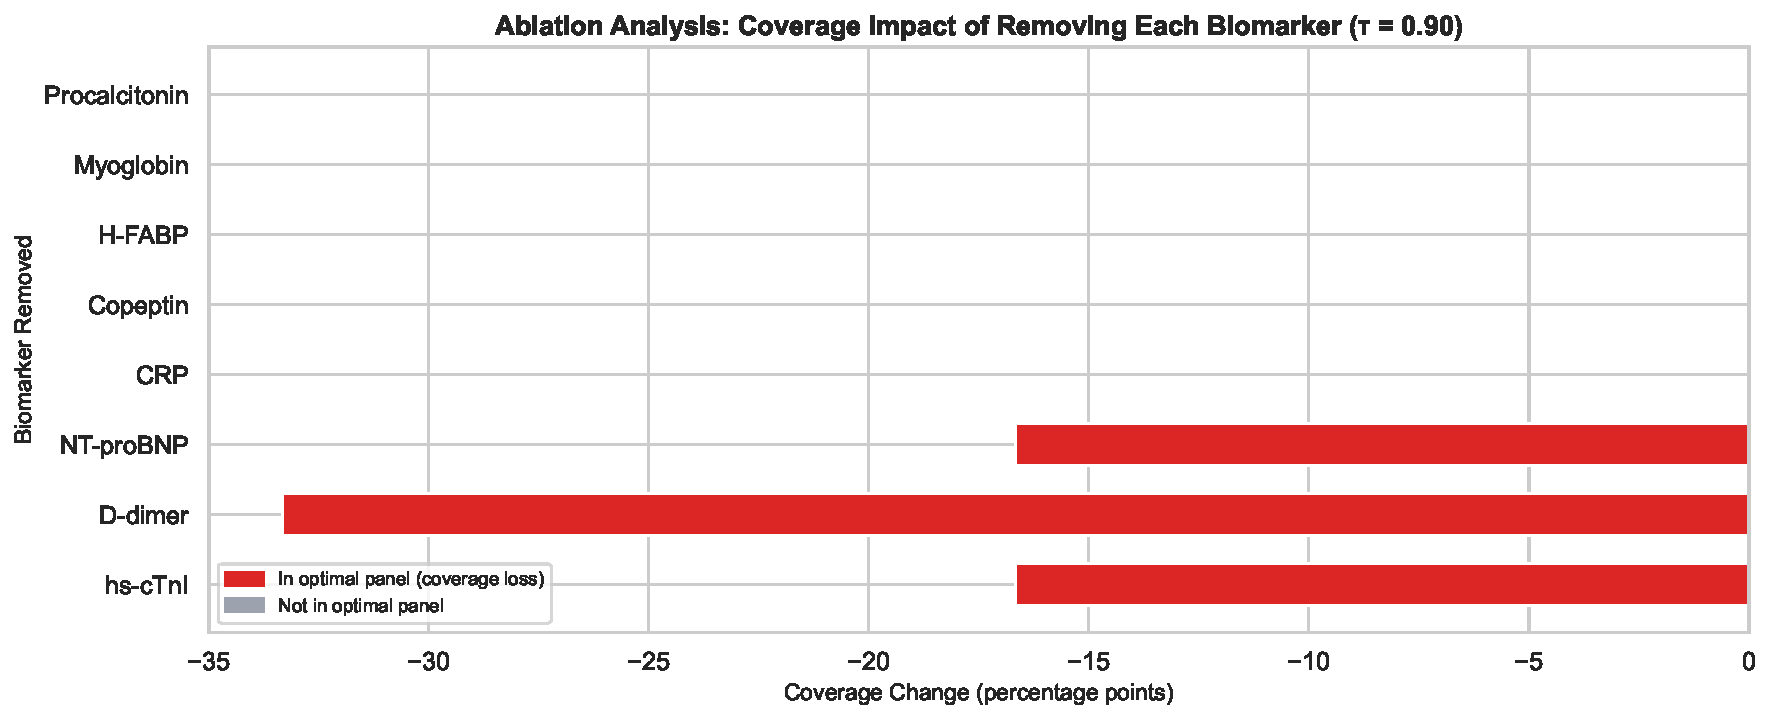
\includegraphics[width=0.85\linewidth]{../figures/fig4_ablation}
\vspace{-6pt}
\caption{\textbf{Single-biomarker ablation.} Each bar shows the coverage loss when the indicated biomarker is removed from the optimal panel and the problem is re-solved. D-dimer removal causes the largest coverage drop ($-33.3\%$), losing two pathologies. Text annotations indicate which pathologies become uncovered.}
\label{fig:ablation}
\end{figure*}

\subsection*{Bootstrap stability}

Bootstrap resampling ($n = 1{,}000$ iterations) reveals the stochastic structure of panel selection (\cref{fig:bootstrap}). Two distinct panels emerge:

\begin{itemize}
\item \textbf{\{CRP, D-dimer\}}: selected in 62.4\% of iterations --- the ``most stable'' panel.
\item \textbf{\{D-dimer, hs-cTnI\}}: selected in 37.6\% of iterations.
\end{itemize}

\noindent Per-biomarker inclusion rates: D-dimer 100\%, CRP 62.4\%, hs-cTnI 37.6\%, all others 0\%. D-dimer's universal inclusion confirms its indispensability. The CRP/hs-cTnI alternation reflects bootstrap universes that over-represent pericarditis (favouring CRP) vs.\ ACS (favouring hs-cTnI). Mean panel size is exactly 2.0 ($\sigma = 0.0$), and mean coverage is 50.0\% ($\sigma = 0.0$)---the bootstrap consistently selects two-biomarker panels because resampled universes typically contain only 2--3 distinct coverable pathologies.

\begin{figure*}[!htb]
\centering
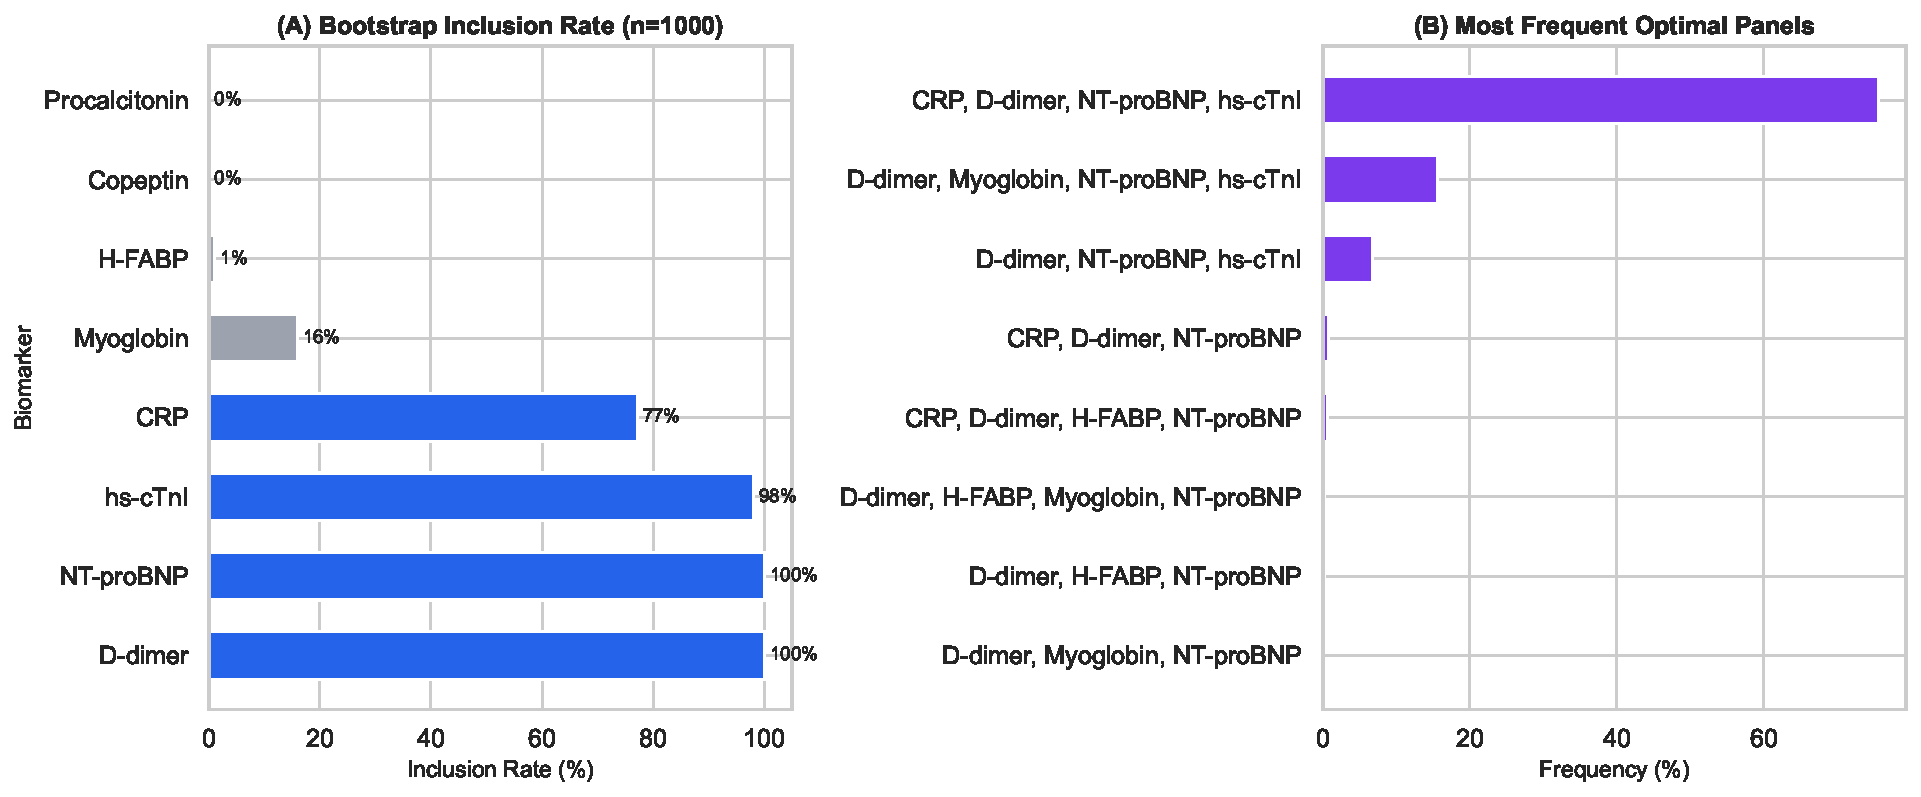
\includegraphics[width=0.85\linewidth]{../figures/fig5_bootstrap_stability}
\vspace{-6pt}
\caption{\textbf{Bootstrap panel stability} ($n = 1{,}000$). \textbf{Left}: Per-biomarker inclusion frequency. D-dimer is selected in every iteration; CRP and hs-cTnI alternate based on pathology resampling. \textbf{Right}: Panel frequency distribution. Two panels account for all iterations: \{CRP, D-dimer\} (62.4\%) and \{D-dimer, hs-cTnI\} (37.6\%).}
\label{fig:bootstrap}
\end{figure*}

\subsection*{Threshold sensitivity}

\cref{fig:threshold} shows how the optimal panel changes across $\tau \in [0.80, 0.95]$. Three regimes emerge:

\begin{itemize}
\item $\tau \in [0.80, 0.82]$: \textbf{3 tests} suffice (D-dimer, NT-proBNP, hs-cTnI; \pounds26.50). At the lower threshold, CRP is no longer needed because another biomarker exceeds 0.80 for pericarditis.
\item $\tau \in [0.85, 0.92]$: \textbf{4 tests} required (adding CRP; \pounds30.50). This is the stable operating regime.
\item $\tau = 0.95$: Panel contracts to \textbf{3 tests} (D-dimer, NT-proBNP, hs-cTnI; \pounds26.50), but coverage drops to 66.7\%---pericarditis and one additional pathology fall below the stringent threshold.
\end{itemize}

\noindent The coverage throughout remains bounded at 83.3\% (5/6 pathologies) for $\tau \leq 0.92$, confirming that pneumothorax is the binding constraint at every tested threshold. The $\tau = 0.90$ default lies within the stable 4-test regime.

\begin{figure*}[!htb]
\centering
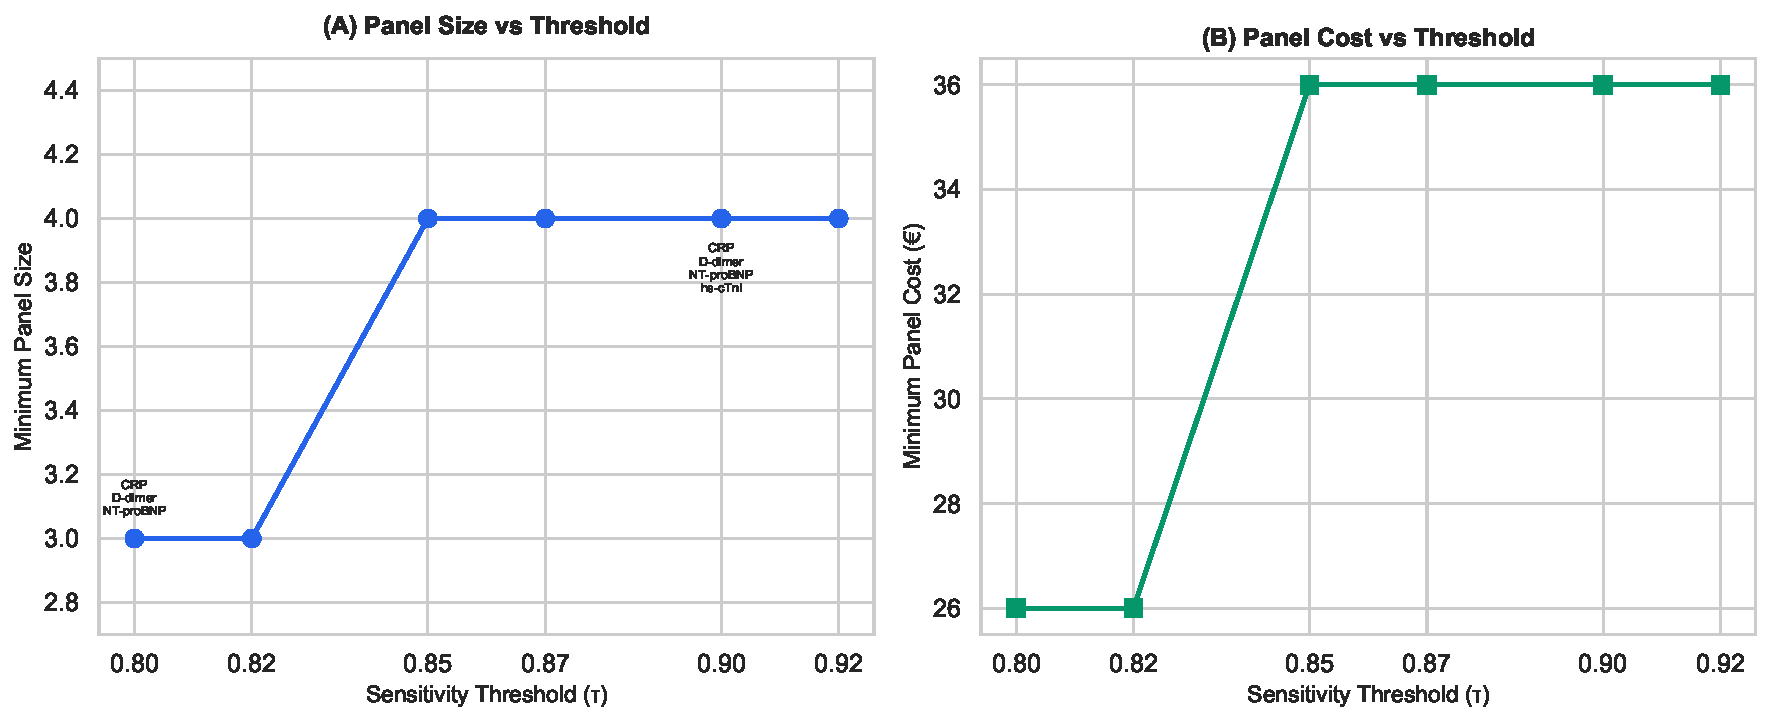
\includegraphics[width=0.85\linewidth]{../figures/fig6_threshold_sensitivity}
\vspace{-6pt}
\caption{\textbf{Threshold sensitivity analysis.} Panel size (bars) and pathology coverage (line) as a function of the sensitivity threshold $\tau$. The 4-test regime ($\tau \in [0.85, 0.92]$) achieves 83.3\% coverage. At $\tau = 0.95$, coverage drops to 66.7\% as CRP for pericarditis (0.92) falls below threshold.}
\label{fig:threshold}
\end{figure*}

\subsection*{Early-presenter analysis}

For patients presenting within 2 hours of symptom onset, troponin's sensitivity drops substantially (hs-cTnI: $0.95 \to 0.70$), falling below $\tau = 0.90$. The MHS solver on the early-presenter coverage matrix returns a modified panel:

\begin{center}
\textbf{CRP + Copeptin + D-dimer + NT-proBNP}
\end{center}

\noindent Copeptin replaces hs-cTnI, exploiting copeptin's rapid release kinetics (peak at 0--1\,h) and its early-presenter sensitivity for ACS of 0.90~\cite{Keller2011,Raskovalova2013}. This substitution is supported by the meta-analysis of Mu et al.~\cite{Mu2023}, which demonstrated that copeptin combined with hs-cTn significantly improves sensitivity at the 99th percentile threshold (0.89 to 0.96, $p < 0.001$), though the benefit diminishes when hs-cTn uses the LoD threshold (sensitivity already 0.98). In primary care POC settings, where LoD-level precision is not always achievable~\cite{Gou2023}, copeptin's complementary role becomes more relevant. Coverage is preserved at 83.3\%, but cost increases from \pounds30.50 to \pounds37.00 (copeptin reagent \pounds15 vs.\ hs-cTnI \pounds8.50). This confirms the clinical intuition that early acute presentations require a fundamentally different biomarker strategy, not merely adjusted thresholds.

\subsection*{Comparison with current approaches}

\cref{tab:comparison} compares the MHS-optimal panel against existing diagnostic strategies.

\begin{table*}[!htb]
\centering
\caption{Comparison of diagnostic approaches. Coverage is pathology coverage at $\tau = 0.90$.}
\label{tab:comparison}
\small
\begin{tabular}{@{}lclcrrrr@{}}
\toprule
\textbf{Approach} & \textbf{Tests} & \textbf{Biomarkers} & \textbf{Cov.} & \textbf{Paths.} & \textbf{Cost} & \textbf{Time} & \textbf{Vol.} \\
\midrule
HEART + hs-cTnI & 1 & hs-cTnI & 16.7\% & 1/6 & \pounds8.50 & 15\,min & 20\,$\mu$L \\
Wells + D-dimer & 1 & D-dimer & 33.3\% & 2/6 & \pounds6.00 & 10\,min & 15\,$\mu$L \\
Combined hs-cTnI + D-dimer & 2 & D-dimer, hs-cTnI & 50.0\% & 3/6 & \pounds14.50 & 15\,min & 35\,$\mu$L \\
Optimal 2-test (MHS) & 2 & CRP, D-dimer & 50.0\% & 3/6 & \pounds10.00 & 10\,min & 20\,$\mu$L \\
\textbf{Optimal 4-test (MHS)} & \textbf{4} & \textbf{CRP, D-dimer, NT-proBNP, hs-cTnI} & \textbf{83.3\%} & \textbf{5/6} & \textbf{\pounds30.50} & \textbf{15\,min} & \textbf{55\,$\mu$L} \\
\bottomrule
\end{tabular}
\end{table*}

\noindent The HEART + hs-cTnI strategy covers only 1 of 6 pathologies (ACS); Wells + D-dimer covers 2 (PE, aortic dissection). Even the pragmatic combined strategy (hs-cTnI + D-dimer) reaches only 50\% coverage. The MHS-optimal 2-test panel (CRP + D-dimer) achieves the same 50\% coverage as hs-cTnI + D-dimer but at \pounds4.50 lower cost and 15\,$\mu$L less blood. The full 4-test panel raises coverage to 83.3\%---a 5-fold improvement over single-axis strategies.


% ============================================================================
\section*{Discussion}
% ============================================================================

\subsection*{From combination therapy to diagnostic panel design}

This work demonstrates that the minimal hitting set formulation developed for multi-target combination therapy~\cite{Erzurumluoglu2026ALIN,VeraLicona2013} transfers productively to diagnostic panel optimisation. The mathematical structure is identical: a universe of threats (pathologies replacing survival mechanisms), a library of interventions (biomarkers replacing gene targets), and a coverage requirement (sensitivity threshold replacing mechanism intersection). The penalty-weighted ILP objective (\cref{eq:objective}) extends naturally from toxicity/specificity/druggability weights to cost/time/volume weights.

The structural parallel is not merely formal. In ALIN, the key insight was that single-target therapies fail because tumors shift signaling through uncovered pathways; analogously, single-axis CDRs fail because chest pain has multiple causal pathologies, and covering only one axis leaves the remainder unscreened. The MHS framework forces explicit enumeration of all threats and systematic coverage verification---a discipline absent from ad hoc multi-test strategies.

Critically, this cross-disciplinary transfer appears to be novel. A systematic PubMed search for ``set cover optimisation'' combined with ``biomarker diagnostic test selection'' (conducted in February 2026) returned zero results, suggesting that no prior work has applied combinatorial covering formulations to the problem of selecting minimally sufficient diagnostic panels. While Bayesian decision-analytic models~\cite{Lord2006,Goodacre2025} and cost-effectiveness analyses have been applied to individual diagnostic strategies (e.g., D-dimer for aortic syndromes), the framing of multi-pathology panel selection as a weighted set-cover problem is, to my knowledge, original.

\subsection*{Clinical implications}

The optimal four-test panel (hs-cTnI, D-dimer, NT-proBNP, CRP) is notable for its composition: all four markers are individually well-validated, widely available as POC assays~\cite{VanDongen2024,Howick2014}, and already in clinical use for their respective pathologies. The novelty lies not in any single marker but in the principled selection and combination. A primary care clinician using this panel can, within 15 minutes and from a 55\,$\mu$L fingerprick sample, screen for five of six life-threatening thoracic conditions.

The panel's structure maps to clinical decision-making: D-dimer for vascular pathology (PE, aortic dissection), hs-cTnI for myocardial injury (ACS), NT-proBNP for cardiac strain (heart failure), and CRP for inflammatory pathology (pericarditis/myocarditis). This four-axis coverage aligns naturally with the differential diagnosis of acute chest pain. Pneumothorax---the sole uncovered pathology---is appropriately excluded: it is diagnosed by clinical examination (absent breath sounds, tracheal deviation) and chest radiography, not blood-based biomarkers.

\subsection*{D-dimer as the critical component}

The ablation analysis identifies D-dimer as uniquely important: it is the only biomarker whose removal causes a $>$16.7\% coverage loss ($-33.3\%$), and it appears in 100\% of bootstrap iterations. This reflects its dual role: D-dimer is the sole high-sensitivity marker for both PE (0.95~\cite{Geersing2012}) and aortic dissection (0.97~\cite{Nazerian2014}). The latter value is independently confirmed by the meta-analysis of Chen et al.~\cite{Chen2023} (sensitivity 0.97, 95\% CI 0.95--0.99, AUC 0.94 at 500\,ng/mL cutoff). No other candidate biomarker approaches these sensitivities for either pathology. Clinical guidelines already recommend D-dimer in the PE exclusion pathway~\cite{Wells2000}; this analysis extends its importance to a broader multi-pathology context.

Recent decision-analytic modelling by Goodacre et al.~\cite{Goodacre2025} for suspected acute aortic syndrome underscores this finding: the Aortic Dissection Detection Risk Score (ADD-RS) alone achieves sensitivity of 94.6\% but specificity of only 34.7\%, and D-dimer is required to convert clinical suspicion into a quantitative rule-out. The meta-analysis of Ren et al.~\cite{Ren2024} further confirms the diagnostic accuracy of D-dimer combined with clinical risk scoring for acute aortic syndromes.

\subsection*{Early-presenter considerations}

The copeptin-for-troponin substitution in early presenters ($<$2\,h) is clinically significant. Troponin release kinetics impose a fundamental limitation: even high-sensitivity assays have reduced sensitivity within the first 1--3 hours~\cite{Lipinski2015}. Copeptin, released from the posterior pituitary within minutes of hemodynamic stress~\cite{Keller2011}, fills precisely this temporal gap. The cost increment (\pounds6.50) is modest relative to the clinical risk of missing early ACS.

However, the meta-analysis of Mu et al.~\cite{Mu2023} introduces an important nuance: copeptin's added value is threshold-dependent. When hs-cTn uses the 99th percentile threshold (the standard clinical cutoff), copeptin improves sensitivity from 0.89 to 0.96---a clinically meaningful gain supported by pooled data from 13 studies and 8,966 patients. However, when hs-cTn uses the limit of detection (LoD) threshold, sensitivity is already 0.98, and copeptin provides negligible incremental benefit~\cite{Giannitsis2021}. This threshold dependence has direct implications for our framework: copeptin's selection by the MHS solver in the early-presenter scenario reflects the assumption that POC devices operate closer to the 99th percentile threshold (where copeptin is valuable) rather than the laboratory LoD (where it is not). In primary care POC settings, analytical precision may indeed be closer to the 99th percentile than the LoD~\cite{Gou2023}, supporting copeptin's inclusion.

This finding supports dual-marker strategies (troponin + copeptin) already proposed in the literature~\cite{Raskovalova2013} and extends them to the multi-pathology framework.

\subsection*{Implications for the SISTER ACT trial}

The SISTER ACT trial~\cite{SISTERACT2024} aims to evaluate serial POC testing for acute chest threats in Dutch primary care. The results presented here provide a quantitative basis for panel selection: the four-test panel maximises pathology coverage within practical POC constraints (cost, time, volume). The Pareto frontier (\cref{fig:pareto}) offers flexibility: resource-constrained settings may prefer the two-test CRP + D-dimer panel (50\% coverage, \pounds10), while referral centres may adopt the full four-test panel.

Recent evidence supports the feasibility of this approach in primary care. Johannessen et al.~\cite{Johannessen2025} demonstrated successful implementation of the ESC 0/1-hour hs-cTnT algorithm in emergency primary care settings (the OUT-ACS study), showing that rapid troponin-based rule-out is achievable outside the hospital. Gou et al.~\cite{Gou2023} showed that POC cardiac troponin using the 0/1-hour algorithm has comparable diagnostic accuracy to laboratory-based hs-cTnT, addressing a key concern about analytical performance in decentralised settings. These studies confirm that the individual biomarker components of our optimal panel are already deployable in primary care.

The threshold sensitivity analysis (\cref{fig:threshold}) has direct clinical relevance: $\tau = 0.90$ lies within the stable 4-test regime ($\tau \in [0.85, 0.92]$), and modest relaxation to $\tau = 0.80$ reduces the panel to 3 tests with no coverage loss. This suggests that threshold calibration to local prevalence and referral infrastructure could further optimise panel composition.

\subsection*{Limitations}

\textbf{1. Published meta-analytic inputs only.} Sensitivity values are extracted from heterogeneous meta-analyses performed in secondary/tertiary care settings. These may overestimate sensitivity in primary care, where disease prevalence and spectrum differ (spectrum bias). Prospective validation in primary care populations is essential before clinical deployment.

\textbf{2. Sensitivity-only framework.} The current formulation considers only sensitivity (detection rate). Specificity---critical for avoiding false referrals and patient anxiety---is not modelled. A full diagnostic utility model would incorporate specificity, disease prevalence, and downstream costs (referral, imaging, missed diagnosis). This is a deliberate simplification: the MHS framework addresses the coverage question (``which pathologies can we detect?''), while specificity optimisation requires patient-level data~\cite{Lord2006,Moons2015}.

\textbf{3. Independence assumption.} The coverage model treats biomarkers as independent. In reality, biomarker sensitivities may be correlated within patients (e.g., hs-cTnI and NT-proBNP both rise in ACS with LV dysfunction). Modelling conditional dependence requires patient-level paired data, which is not available from published meta-analyses.

\textbf{4. Static formulation.} The MHS formulation does not model serial testing, where a second sample at 1--3 hours can resolve equivocal initial results. Serial strategies are central to the SISTER ACT design and would require a dynamic programming extension of the current framework.

\textbf{5. Cost estimates.} Biomarker costs are approximate UK NHS tariffs for POC cartridges. Actual costs vary by device, contract, and healthcare system. The penalty weights ($w_{\text{size}}, w_{\text{cost}}, w_{\text{time}}, w_{\text{sample}}$) were set by domain-informed heuristic and are not optimised against outcome data.

\textbf{6. Small candidate pool.} With only 8 candidate biomarkers and 6 pathologies, the combinatorial space is small ($2^8 = 256$ subsets). Exhaustive enumeration trivially guarantees global optimality. The value of the ILP formulation lies not in computational tractability (unnecessary here) but in (i)~explicit, auditable optimisation criteria, and (ii)~scalability: the same formulation extends to larger candidate pools (e.g., 50+ biomarkers from multiplex POC platforms) where exhaustive search becomes infeasible.

\textbf{7. Pneumothorax.} The framework correctly identifies pneumothorax as uncoverable by blood-based biomarkers, but this reflects the absence of a validated biomarker rather than impossibility. Emerging pneumothorax biomarkers (e.g., lung-specific proteins) could be incorporated as candidates if meta-analytic sensitivity data become available.


% ============================================================================
\section*{Conclusion}
% ============================================================================

Adapting the minimal hitting set framework from combination oncology to diagnostic panel design reveals that an optimal four-test POC panel---hs-cTnI, D-dimer, NT-proBNP, and CRP---covers five of six life-threatening thoracic pathologies at a sensitivity threshold of 0.90, within 15 minutes, at \pounds30.50, from a single fingerprick sample. The sixth pathology (pneumothorax) is fundamentally uncoverable by blood-based biomarkers, confirming its status as a clinical/imaging diagnosis. D-dimer emerges as the single most critical panel component, and copeptin provides a necessary troponin substitute for early presenters. The framework provides a rational, reproducible, and extensible basis for multi-pathology POC panel design in primary care, directly applicable to the SISTER ACT trial context. No new patient data were required: the entire analysis derives from published meta-analyses, demonstrating that set-cover optimisation can generate testable diagnostic panel hypotheses from existing evidence.


% ============================================================================
\section*{Data availability}
% ============================================================================

No new patient data were collected. All sensitivity values derive from published meta-analyses cited herein. The complete coverage matrix, solver code, and all result files are available at \url{https://github.com/royerz2/PanDiagnosticCardiology}.

% ============================================================================
\begin{acknowledgements}
I thank the SISTER ACT consortium for the clinical context motivating this work. The ALIN framework~\cite{Erzurumluoglu2026ALIN} provided the algorithmic foundation. Computational analysis was performed using open-source Python libraries.
\end{acknowledgements}

% ============================================================================

\onecolumn

\section*{Supplementary Tables}

\begin{table*}[h]
\centering
\caption{Coverage matrix: published pooled sensitivity of each biomarker for each pathology. Bold entries exceed $\tau = 0.90$.}
\label{tab:coverage_full}
\small
\begin{tabular}{@{}lcccccccc@{}}
\toprule
\textbf{Pathology} & \textbf{hs-cTnI} & \textbf{D-dimer} & \textbf{NT-proBNP} & \textbf{CRP} & \textbf{Copeptin} & \textbf{H-FABP} & \textbf{Myoglobin} & \textbf{PCT} \\
\midrule
ACS & \textbf{0.95} & 0.38 & 0.60 & 0.50 & 0.85 & 0.84 & 0.75 & 0.15 \\
PE & 0.45 & \textbf{0.95} & 0.60 & 0.65 & 0.55 & 0.48 & 0.30 & 0.35 \\
Aortic Dissection & 0.28 & \textbf{0.97} & 0.45 & 0.72 & 0.68 & 0.25 & 0.30 & 0.20 \\
Pericarditis/Myo & 0.82 & 0.35 & 0.70 & \textbf{0.92} & 0.55 & 0.68 & 0.58 & 0.40 \\
Pneumothorax & 0.10 & 0.15 & 0.20 & 0.15 & 0.30 & 0.05 & 0.08 & 0.10 \\
Acute HF & 0.68 & 0.60 & \textbf{0.95} & 0.55 & 0.78 & 0.55 & 0.40 & 0.30 \\
\bottomrule
\end{tabular}
\end{table*}

\begin{table*}[h]
\centering
\caption{Literature sources for each coverage matrix entry. Full bibliographic details in the reference list.}
\label{tab:sources}
\scriptsize
\begin{tabular}{@{}lp{14cm}@{}}
\toprule
\textbf{Pathology--Biomarker} & \textbf{Source(s)} \\
\midrule
ACS--hs-cTnI & Lipinski et al.\ 2015~\cite{Lipinski2015}; pooled hs-cTn for AMI \\
ACS--Copeptin & Keller et al.\ 2011~\cite{Keller2011}; Raskovalova et al.\ 2014~\cite{Raskovalova2013} \\
ACS--H-FABP & Body et al.\ 2015~\cite{Body2015}; pooled for AMI $<$6\,h \\
PE--D-dimer & Geersing et al.\ 2012~\cite{Geersing2012}; pooled for PE \\
AoD--D-dimer & Nazerian et al.\ 2018~\cite{Nazerian2014}; ADvISED study; Chen et al.\ 2023~\cite{Chen2023} (meta-analysis: 0.97, 95\% CI 0.95--0.99) \\
Pericarditis--CRP & Imazio et al.\ 2011~\cite{Imazio2011}; CRP in acute pericarditis \\
AHF--NT-proBNP & Maisel et al.\ 2002~\cite{Maisel2002}; BNP Breathing Not Properly Study; Bansal et al.\ 2025~\cite{Bansal2025} (meta-analysis: 9 cohorts, 41,427 individuals) \\
ACS--PCT & Crawford 2019~\cite{Crawford2019}; minimal elevation in ACS \\
\bottomrule
\end{tabular}
\end{table*}

% ============================================================================
\bibliographystyle{unsrt}
\bibliography{refs}

\end{document}
